\documentclass[a4paper,norsk]{article}
\usepackage[utf8]{inputenc}
\usepackage[T1]{fontenc,url}
\usepackage{babel,textcomp}
\usepackage{graphicx, wrapfig}
\usepackage{graphics}
\graphicspath{
	{Code/figs/}
	{Code/scorefigs/}
}
\usepackage{cite}
\usepackage{amsmath}
\usepackage{bm}
\usepackage{stackengine}
\usepackage{listings}
\usepackage{amsfonts}
\urlstyle {sf}
\title {Project 1 FYS-STK4155 Autumn 2018}
\author {Jon Audun Baar \& Mikael Ravndal}
\begin{document}
\maketitle
%All of the plots of the models are done with degree equals 5.

\section{Introduction}
A common problem in inferential statistics is to investigate how one 
stocastic variable depends on another stocastic variable. That is, one
wishes to find a model that given the outcome of one stocastic variable 
estimates the outcome of another stocastic variable.
A widely used technique for developing such a model is a method called 
linear regression. In this project 
we aim to evaluate the performance of three different types of 
linear regression using a polynomial as our model. The methods are:
ordinary least squares regression (abreviated OLS), ridge regression and
lasso regression.
\par First we evaluate our methods on a known function, that is we know 
the relationship between our variables. Then we apply the same methods 
to evaluate the performance of our methods on a real data set where 
we don’t know the underlying relationship (if there is any at all).
%In this project we were to analyse different sets of data; test-data 
%from the Franke-function and real data, using different linear 
%regression models. The main goal of the project was to evaulate the 
%different models, and come to a conclusion in terms of which models 
%would fit best with which data.

\section{Method}
The general idea of linear regression is to assume that the relationship 
between your dependent and independent variables is given by some function 
(which is linear in it's coefficients)
and then try to estimate this function, also called a model, 
by minimizing some error term. As the scope of this text is to evaluate the
goodnes of this method in some special cases rather than explaining it 
in general, we are not going to induldge in the derivation of this method
but rather assume that the reader is familiar with the basics of this
concept. However we will need to establish some context and 
notation.
\par
In our case we are given two independent variables, also called 
\textit{predictors}, 
and one dependent variable, also called 
\textit{response}. We denote by 
$N$ the number of 
datapoints/observations in our sampledata and gather the observations 
of the predictors in two vectors $\bm{x_1} \in \mathbb{R}^N$ and 
$\bm{x_2} \in \mathbb{R}^N$, and the observations of the response in one 
vector $\bm{y} \in \mathbb{R}^N$.
\par
Further we assume the true relationship between the predictors and 
response to be:
\begin{equation}
    y = f(x_1, x_2) + \epsilon
\end{equation}
where $\epsilon$ is a stocastic variable which is normally distributed 
around 0 and $f$ is some function. 
We will try to model the function $f$ by a polynomial $p$ of degree $k$ 
given by 
\begin{equation}
    \begin{split}
        p(x_1, x_2) = \ &\beta_0 \ + \\ 
        & \beta_1 x_1 \ + \ \beta_2 x_2 \ + \\
        & \beta_3 x_1^2 \ + \ \beta_4 x_1 x_2 \ + \ \beta_5 x_2^2 \\
        & + \ \dots \ + \\
        & \beta_{q-(k+1)} x_1^k \ + \ \beta_{q-k} x_1^{k-1} x_2 \ 
        + \ \dots \ + \ \beta_{q-1} x_1 x_2^{k-1} \ + \ \beta_q x_2^k
    \end{split}
\end{equation}
Here q is the sum of the natural numbers from $1$ to $k + 1$. We call
$p$ our \textit{model}.
\par
If we let $x_{i,j}$ be the j-th entry of $\bm{x_i}$ 
our design matrix is then given by
\begin{equation}
    X \ = \
    \begin{bmatrix}
        1 &x_{1,1} &x_{2,1} &x_{1,1}^2 &x_{1,1}x_{2,1} &x_{2,1} 
        &\dots &x_{1,1}x_{2,1}^{k-1} &x_{2,1}^k \\
        1 &x_{1,2} &x_{2,2} &x_{1,2}^2 &x_{1,2}x_{2,2} &x_{2,2} 
        &\dots &x_{1,2}x_{2,2}^{k-1} &x_{2,2}^k \\
        \vdots &\vdots & & & & & & &\vdots \\
        1 &x_{1,n} &x_{2,n} &x_{1,n}^2 &x_{1,n}x_{2,n} &x_{2,n} 
        &\dots &x_{1,n}x_{2,n}^{k-1} &x_{2,n}^k
    \end{bmatrix}
\end{equation}
and from what we have established so far we get the equation
\begin{equation}
    \bm{y} = X\bm{\beta} + \bm{\epsilon}
\end{equation}
where $\bm{\epsilon}$ is a vector of errors. Solving this equation for 
$\bm{\epsilon}$, we get that 
$\bm{\epsilon} \ = \ \bm{y} - X\bm{\beta}$.
\par
In the following we will discuss how to estimate $\bm{\beta}$ 
in order to obtain our model $p$. The general idea is the same for 
all three methods: 
we will try to get a good fit of our model to the sample data
by minimizing the magnitude of the vector $\bm{\epsilon}$. In doing this 
we define a function $C:=C(\bm{\beta})$ called the 
\textit{cost function}, which we wish to minimize.

\subsection{Ordinary least squares regression}
In the case of OLS regression the cost function is defined by 
\begin{equation}
    C(\bm{\beta}) = \sum_{i=1}^N (y_i - (X\bm{\beta})_i)^2
\end{equation}
One great benefit of this method as opposed to for instance the 
later explained lasso method, is that the problem of minimizing $C$ over
all $\bm{\beta} \in \mathbb{R}^N$ has an analytical solution. 
One can with some elementary calculus show that the solution is 
given by (6) given that $X$ is non-singular. 
For a thorough explanation of this identity consult \cite{hastie}
\begin{equation}
    \bm{\beta} \ = \ (X^TX)^{-1}X^T\bm{y}
\end{equation}

\subsection{Ridge regression}
One major weakness of OLS regression is that noisy sample data can cause
large coefficients, that is a model with large variance. One way
to approach this problem is to impose a restriction to the magnitude of 
our coefficients $\bm{\beta}$. Ridge regression does this by adding the 
2-norm of $\bm{\beta}$ to the cost function of OLS regression, and in 
that way penalizing large betas. We call this term a \textit{penality}.
The Ridge cost function is therefore given by
\begin{equation}
    C(\bm{\beta}) = \sum_{i=1}^N (y_i - (X\bm{\beta})_i)^2 + 
    \sum_{i=1}^N \beta_i^2
\end{equation}
\par
As with the case of OLS, we are in a good position with respect to solving
this minimization problem. By applying the method of Lagrange multipliers
one can show that the solution for $\bm{\beta}$ is given by
\begin{equation}
    \bm{\beta} \ = \ (X^TX + \lambda I)^{-1}X^T\bm{y}
\end{equation}
where $I$ is the identity matrix and $\lambda$ is a positive real number.
Choosing $\lambda$ big then more emphazises restricting the magnitude of 
$\bm{\beta}$, while choosing a small $\lambda$ more emphazises
minimizing the magnitude of $\bm{\epsilon}$.

\subsection{Lasso regression}
Just as for ridge, the lasso method solves the problem of high variance 
by adding a penality to the cost function. The difference is that 
lasso adds the 1-norm of $\bm{\beta}$ to $C$ instead of the 2-norm. 
Thus we get
\begin{equation}
    C(\bm{\beta}) = \sum_{i=1}^N (\bm{y_i} - \bm{y'_i})^2 + 
    \sum_{i=1}^N |\beta_i|
\end{equation}
The advantage of this approach over ridge 
is that it tends to set coefficients that are irellevant to zero instead
of very small values. One might then end up with a smarter model with 
fewer predictors than one started out with. For a thorough explanation 
of this consult \cite{hastie}. 
The draw back however is that we no longer have an analytical solution for
$\bm{\beta}$ and have to resort to numerical methods to minimize $C$. 

\subsection{Measure of goodnesssssssss}
\subsubsection{Decomposition of MSE}
The standard way of measruing how well

\subsubsection{R2 score}

\subsubsection{Variance, and more parameters?}


\subsubsection{Resampling using bootstrapping}
\par convergence to the real parameteres using bootstrap

\section{Implementation}
We implemented the process described in section 2 using python. 
The complete code can be found in \cite{hastie}. The main part of the code
are the classes OLSLinearModel, RidgeLinearModel and LassoLinearModel. 

We found the choice of implementing our three different models as classes 
a rather intuitive and oversiktlig way of doing it. The advantage of this
implementation is obviously that as we store most of the data in the model
computing the same numbers over again and thus excessive comupting is not
a problem. The weakness might then be excessive memory usage. This was 
hovewer not a problem in our application of the program.

\par Most of our code is in the GitHub repository. We have chosen to 
not use the code in our report. We have, however, made a python file, 
project01.py, that provides most of our code in sequence, 
so that it is possible to follow the code that produce our testresults 
and plots in order.
\subsection{Ordinary least square on the Franke function}

First we have generated some test data, with the noise being very little, 
which we have plotted to get a more intuitive feel for how it looks. 
We have done this for all the models.
\\Ordinary Least square of the Frankefunction(the same as Ridge with $\lambda=0$):
\\ 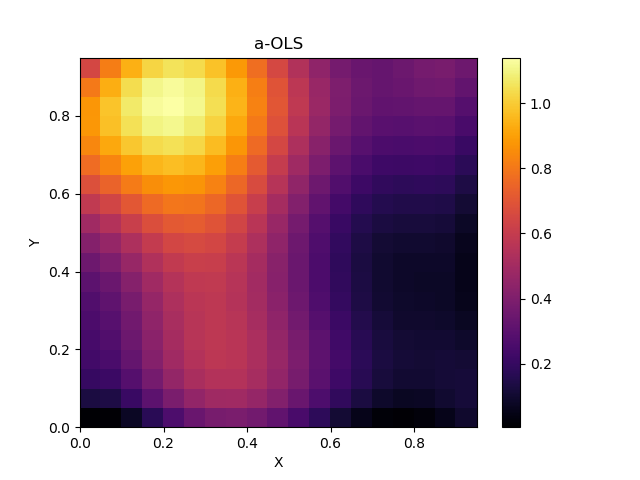
\includegraphics[scale=.7]{a-OLS}
\\As you can tell from our code, we haven't made an own function for ordinary least square, since it is the same as Ridge, just with the $\lambda$ set to 0. This will also show later that when the $\lambda$ gets low it is very similar to OLS.
\\Here is the values for calculating the five first degrees and their MSE and  R2-score:
\\OLS Test Data
\begin{table}[!h]
\begin{tabular}{lll}
k & MSE                   & R2                 \\
1 & 0.020836568820240136  & 0.7159598591230791 \\
2 & 0.015631136506458913  & 0.7869193218104034 \\
3 & 0.007175355204257789  & 0.9021869233537347 \\
4 & 0.003960217232650187  & 0.9460150723293508 \\
5 & 0.0018602479352178107 & 0.9746414541595732
\end{tabular}
\end{table}
We can tell that our model is fitting our test data better and better with a higher degree. Now we have to check with bootstrap as well to see if our model fits the data good.
\\Before the resampling we have also calculated the betas of $k=5$:
\\Var of Beta, degree 5
\begin{align*}
[9.47238055e-03\quad 8.01217226e-01 \quad4.12183842e-01\quad 9.89887798e+00\\
8.39455751e+00\quad 4.14211294e+00\quad 2.71771303e+01\quad 3.28888083e+01\\
1.78285914e+01\quad 1.31093669e+01\quad 1.91368860e+01\quad 2.67004422e+01\\
1.91391193e+01\quad 9.34737951e+00\quad 1.13215581e+01\quad 2.55450522e+00\\
4.40599813e+00\quad 3.60735967e+00\quad 1.80107762e+00\quad 1.00979408e+00\\
1.50021893e+00]
\end{align*}
Also the 95-percentage confidence interval of the betas:
95-percentage CI of betas, degree 5
\begin{align*}
[[ 7.25873511e-02\quad  4.54098870e-01]\\
[ 7.23335269e+00\quad  1.07421092e+01]\\
[ 3.44378188e+00\quad 5.96043621e+00]\\
[-4.41211552e+01\quad -3.17880887e+01]\\
[-2.42828028e+01\quad -1.29254533e+01]\\
[-1.57022805e+01\quad -7.72437196e+00]\\
[ 4.22571363e+01\quad  6.26923830e+01]\\
[ 4.18269196e+01\quad  6.43072224e+01]\\
[ 1.67482166e+01\quad  3.32996879e+01]\\
[-1.02120404e+01\quad  3.98078784e+00]\\
[-3.30453851e+01\quad -1.58973753e+01]\\
[-7.33667324e+01\quad -5.31114961e+01]\\
[-1.94596236e+01\quad -2.31061330e+00]\\
[-3.98768180e+01\quad -2.78922323e+01]\\
[ 1.90552365e+01\quad  3.22448231e+01]\\
[-2.43921072e+00\quad  3.82593943e+00]\\
[ 1.88142647e+01\quad  2.70423776e+01]\\
[ 8.68290825e+00\quad  1.61280472e+01]\\
[-7.84195698e+00\quad -2.58124771e+00]\\
[ 1.66275865e+01\quad  2.05666637e+01]\\
[-1.80168037e+01\quad -1.32155417e+01]]\\
\end{align*}
\\ The code and commenting for the calculations is to be found in python-file project01.py
\subsubsection{Resampling}
Using our bootstrapping algorithm with a resampling of 100, degree of five, we get these values:
\\VAR: 0.000052
\\BIAS: 0.001933
\\Bootstrap mean of MSE: 0.0020
\\Bootstrap mean of r2Score: 0.9757
\\ 
\\The bootsrap values aligns pretty well with our original ones.
\clearpage
\subsection{Ridge regression}
Ridge Regression with $\lambda = 0.1$
\\Graphic plot of how it looks:
\\ 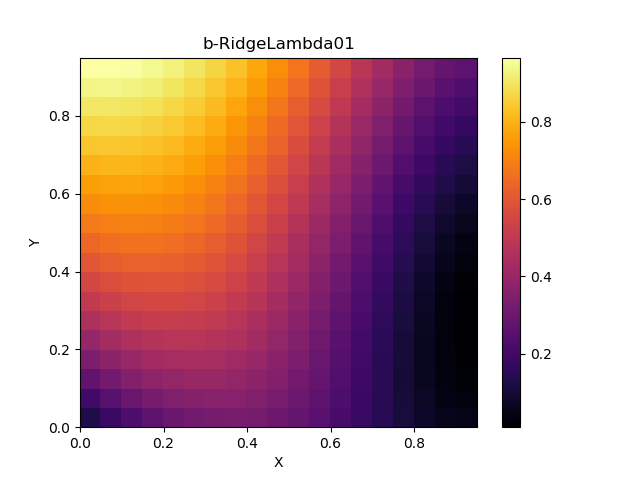
\includegraphics[scale=.7]{b-RidgeLambda01}
\\Ridge Test Data
\begin{table}[!h]
\begin{tabular}{lll}
k & MSE                   & R2                 \\
1 & 0.025965982389446095  & 0.6906471643146342 \\
2 & 0.018247163430545398  & 0.7826074259086047 \\
3 & 0.010258352759015437  & 0.8777843076427536 \\
4 & 0.009382588378732645  & 0.8882179662029949 \\
5 & 0.009143926633340667 & 0.8910613282063765
\end{tabular}
\end{table}
\\Compared to OLS, we can tell that Ridge does significantly worse then OLS.
\\Var of Beta, degree 5
\begin{align*}
[ 0.00077004\quad  0.01729839\quad  0.01384995\quad  0.06816008\quad  0.06826285\quad  0.05696662\\
  0.0417508\quad   0.02034709\quad  0.06671475\quad  0.03500783 \quad 0.02294549\quad  0.01073849\\
  0.03470761\quad  0.01261125\quad  0.02127092 \quad 0.03349824 \quad 0.01062464 \quad 0.03548007\\
  0.03422875\quad  0.04204926\quad  0.02520149]
\end{align*}
Also the 95-percentage confidence interval of the betas:
95-percentage CI of betas, degree 5
\begin{align*}
[[  8.39518095e-01 \quad  9.45603016e-01]\\
   [  6.00189901e-01 \quad  1.10406786e+00]\\
   [  9.22637923e-01 \quad  1.52633094e+00]\\
   [ -6.51421032e+00 \quad -5.30387095e+00]\\
   [  5.84279933e-01 \quad  1.67511842e+00]\\
   [ -5.82384066e+00\quad  -4.85326698e+00]\\
   [  3.42317950e+00 \quad  4.16050815e+00]\\
   [  1.31502300e+00 \quad  2.10193829e+00]\\
   [ -2.00335018e+00\quad  -1.07460992e+00]\\
   [  1.38884378e+00\quad   1.92131292e+00]\\
   [  3.21253289e+00\quad   3.98989176e+00]\\
   [  5.79118852e-01 \quad  1.17557901e+00]\\
   [ -3.41043372e-02 \quad  7.77207310e-01]\\
   [ -8.02285903e-01 \quad -2.23570539e-01]\\
   [  3.31692208e+00\quad   3.80174824e+00]\\
   [ -3.69457810e+00\quad  -2.99905374e+00]\\
   [ -2.10226995e+00\quad  -1.54360569e+00]\\
   [ -5.64130918e-03 \quad  8.94344017e-01]\\
   [ -1.07674065e+00\quad  -1.87377295e-01]\\
   [  3.14047856e-01 \quad  8.79022520e-01]\\
   [ -1.87908328e+00\quad  -1.35609332e+00]]\\
\end{align*}

\subsubsection{Resampling}
We can take a look at how different lambdas and different degrees of the polynomial makes a change in the R2-score and the MSE.
\\Here is a plot to show how they develop as a function of lambda.
\\ 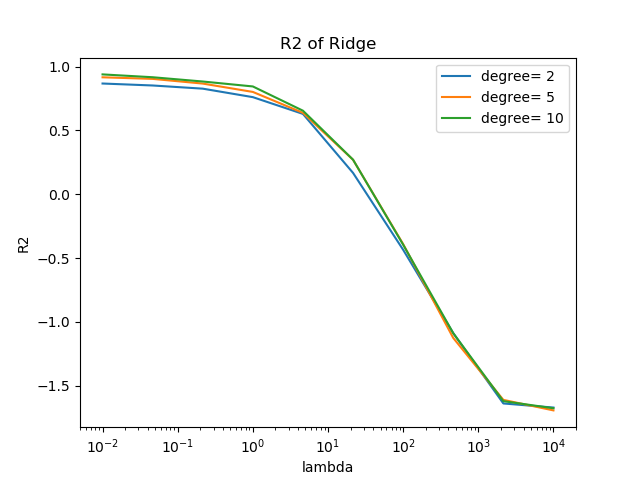
\includegraphics[scale=.7]{R2Ridge}
\\ We can tell pretty easily that the degree of the predictions doesn't matter much compared to how much the choice of lambda do. We can still tell that a lower degree function does worse then the other functions.
\\
\\Some interesting values from bootstrap:
\\
\\Bootstrap-values from degree of 5, lmb = 0.1 and 100 bootstrap-samples
\\VAR: 0.000067
\\BIAS: 0.008640
\\Bootstrap mean of MSE: 0.0087
\\Bootstrap mean of r2Score: 0.8980
\\
\\Bootstrap-values from degree of 5, lmb = 1 and 100 bootstrap-samples
\\VAR: 0.000059
\\BIAS: 0.011915
\\Bootstrap mean of MSE: 0.0120
\\Bootstrap mean of r2Score: 0.8597
\\
\\Bootstrap-values from degree of 5, lmb = 10 and 100 bootstrap-samples
\\VAR: 0.000066
\\BIAS: 0.020274
\\Bootstrap mean of MSE: 0.0203
\\Bootstrap mean of r2Score: 0.7617
\\
\\Bootstrap-values from degree of 2, lmb = 10 and 100 bootstrap-samples
\\VAR: 0.000057
\\BIAS: 0.022754
\\Bootstrap mean of MSE: 0.0228
\\Bootstrap mean of r2Score: 0.7327

\clearpage

\subsection{Part c)}
Lasso Regression with $\lambda = 0.01$
\\ 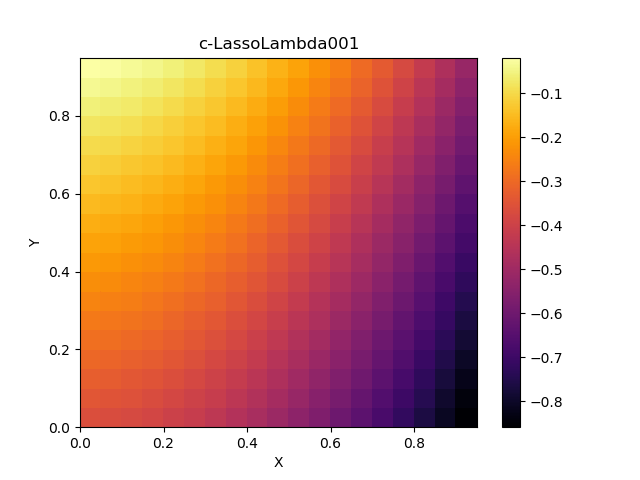
\includegraphics[scale=.7]{c-LassoLambda001}
\\Ridge Test Data
\begin{table}[!h]
\begin{tabular}{lll}
k & MSE                   & R2                 \\
1 & 0.25272407945476655  & -2.01089746779934852 \\
2 & 0.25272407945476655  & -2.0108974677993485 \\
3 & 0.25272407945476655  & -2.0108974677993485 \\
4 & 0.25272407945476655  & -2.0108974677993485 \\
5 & 0.25272407945476655 & -2.0108974677993485
\end{tabular}
\end{table}

Var of Beta
\begin{align*}
[ 0.   \quad       0.00025829 \quad 0.00394575\quad  0.     \quad     0.    \quad      0.00324571\\
  0.      \quad    0.     \quad     0.    \quad      0.    \quad      0.     \quad     0.    \quad      0.\\
  0.     \quad     0.   \quad       0.      \quad    0.     \quad     0.     \quad     0.   \quad       0.\\
  0.        ]
\end{align*}

95-percentage CI of betas
\begin{align*}
[[ 0.      \quad    0.        ]\\
 [-0.40937802\quad -0.34637908]\\
 [-0.17825992\quad  0.06797132]\\
 [-0.      \quad    0.        ]\\
 [-0.   \quad       0.        ]\\
 [-0.58986796\quad -0.36654512]\\
 [-0.    \quad      0.        ]\\
 [-0.   \quad       0.        ]\\
 [-0.    \quad      0.        ]\\
 [-0.   \quad       0.        ]\\
 [-0.     \quad     0.        ]\\
 [-0.     \quad     0.        ]\\
 [-0.   \quad       0.        ]\\
 [-0.    \quad      0.        ]\\
 [-0.    \quad      0.        ]\\
 [-0.    \quad      0.        ]\\
 [-0.     \quad     0.        ]\\
 [-0.    \quad      0.        ]\\
 [-0.    \quad      0.        ]\\
 [-0.   \quad       0.        ]\\
 [-0.    \quad      0.        ]]
\end{align*}
\\There is obviusly something happening with Lasso that doesn't work. Our Lasso method works great with the real data.
\subsubsection{Resampling}
Bootstrap-values from degree of 1, lmb = 0.1 and 100 bootstrap-samples
\\VAR: 0.000000
\\BIAS: 0.239704
\\Bootstrap mean of MSE: 0.2397
\\Bootstrap mean of r2Score: -2.0278
\\This was the same for all degrees and values of lambda, so I only included this.
\clearpage

\subsection{Part d)}
Imports 100x100 chunk of real data from top left corner of dataset nr.1.
\\Plot of real data
\\ 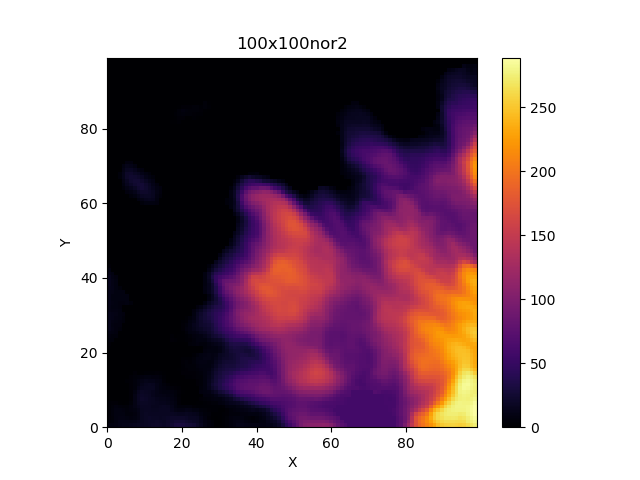
\includegraphics[scale=.7]{100x100nor2}
\clearpage
\subsection{Real Data}
Repeat of the previous method and data, but with real data.
\subsection{OLS}
Plot of the data with the OLS-method of degree 5:
\\ 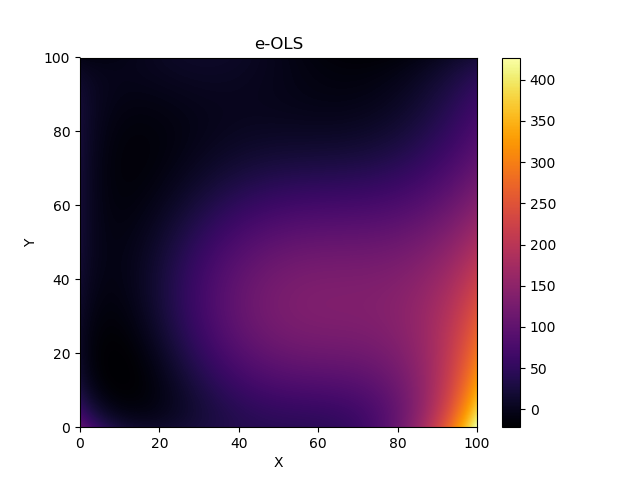
\includegraphics[scale=.7]{e-OLS}
\\ OLS Score of the Real Data:
\begin{table}[!h]
\begin{tabular}{lll}
k & MSE                   & R2                 \\
1 & 1912.190996  & 0.587579 \\
2 & 1177.397306  & 0.746059 \\
3 & 1023.042624  & 0.779351 \\
4 & 824.587589  & 0.822153 \\
5 & 791.268452 & 0.829340
\end{tabular}
\end{table}
\\Var of Beta
\begin{align*}
[  2.32350868e-17\quad   3.59021583e-14 \quad  9.26320612e-14\quad   6.67623760e-12\\
   2.76179532e-12\quad   2.44594128e-11 \quad  1.00899287e-09  \quad 2.82477031e-08\\
   3.26102575e-08 \quad  4.03014136e-09 \quad  7.93068781e-13  \quad 8.29815731e-12\\
   2.72417498e-12 \quad  8.99036913e-12 \quad  2.47909085e-12 \quad  4.07929803e-17\\
   2.67723887e-16 \quad  5.18767547e-16 \quad  4.23509770e-16 \quad  1.84571052e-16\\
   9.42227510e-17]
\end{align*}

\subsubsection{Resampling}
Bootstrap-values from degree of 5 and 100 bootstrap-samples
\\VAR: 1.287057
\\BIAS: 791.273865
\\Bootstrap mean of MSE: 792.5609
\\Bootstrap mean of r2Score: 0.8291
\\
\\The MSE and R2-score are really close to our values for MSE and R2.

\subsection{Ridge}
Plot of the data with the Ridge-method of degree 5, lambda = 0.1:
\\ 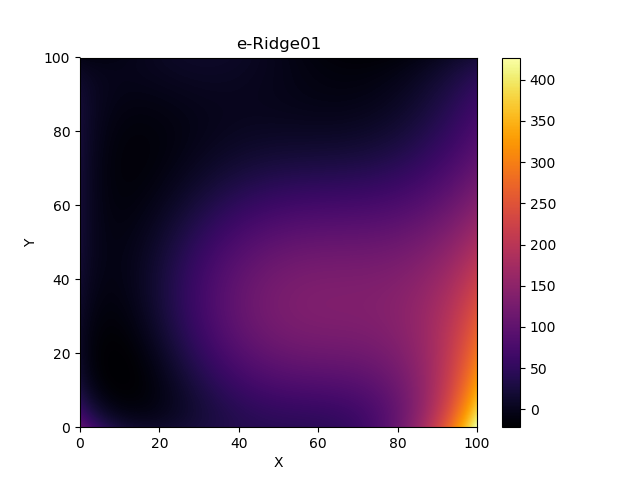
\includegraphics[scale=.7]{e-Ridge01}
\\ Ridge Score of the Real Data with lambda = 0.1:
\begin{table}[!h]
\begin{tabular}{lll}
k & MSE                   & R2                 \\
1 & 1912.190999  & 0.587579 \\
2 & 1177.397307  & 0.746059 \\
3 & 1023.042624  & 0.779351 \\
4 & 824.635824  & 0.822143 \\
5 & 791.268452 & 0.829340
\end{tabular}
\end{table}
\subsubsection{Resampling}
Bootstrap-values from degree of 5, lmb = 10 and 100 bootstrap-samples
\\VAR: 1.297002
\\BIAS: 791.285081
\\Bootstrap mean of MSE: 792.5821
\\Bootstrap mean of r2Score: 0.8291
\\Can tell that MSE and R2-score is pretty similar to our computations.
\subsection{Lasso}
Plot of the data with the Lasso-method of degree 5, lambda = 0.01:
\\ 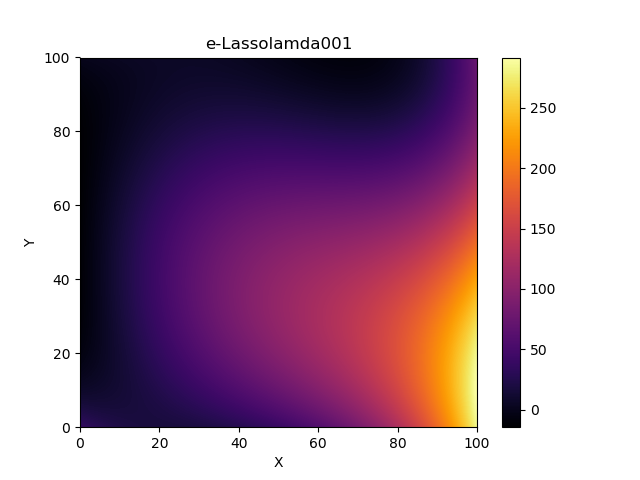
\includegraphics[scale=.7]{e-Lassolamda001}
\\ Lasso Score of the Real Data with lambda= 0.1:
\begin{table}[!h]
\begin{tabular}{lll}
k & MSE                   & R2                 \\
1 & 6601.647721  & -0.423841 \\
2 & 1564.545187  & 0.662560 \\
3 & 1189.660192  & 0.743415 \\
4 & 1155.338990  & 0.750817 \\
5 & 974.391256 & 0.789844
\end{tabular}
\end{table}
\subsubsection{Resampling}
Bootstrap-values from degree of 5, lmb = 10 and 100 bootstrap-samples
\\VAR: 1.689048
\\BIAS: 1239.400793
\\Bootstrap mean of MSE: 1241.0898
\\Bootstrap mean of r2Score: 0.7323
\\
\\Here the MSE and R2score is a pretty long way from our scores when we use all our data. So the model is probably a little overfitted and we should expect our R2 to actually be lower than it is.
\clearpage
\section{Conclusion}

\par
Outlooks, further investigation, etc.

\end{document}
